\chapter{Data recording}
As we have learned in Chapter 2, a diffraction pattern is the Fourier transform of the scattering potential, sampled at the Ewald sphere ($F({\vec{S}})$). This Chapter will describe the essentials of the process of measuring the diffracted signal.

The value of $F(\vec{S})$ is complex. The complex amplitude corresponds to the amplitude of the measured wave, and the complex argument corresponds to the phase shift of the wave. Currently no device exists capable of measuring the phase of x-rays directly, as it changes in the attosecond time range. The amplitude of the electron magnetic wave can be determined, and this is exactly what is recorded in an intensity measurement. 

\begin{equation}
I(\vec{S}) = |F(\vec{S})|^2
\end{equation}
where $I(\vec{S})$ is the measured intensity.

In the experiments described in this thesis we used a pnCCD detector to determine the $I(\vec{S})$. A pnCCD is a 2D array of pixels of size $p$. Each pixel registers the intensity of the electro magnetic wave at that location by converting the energy present in the wave into an electrical current, using a physical process called the photo-electric effect. 

Figure \ref{fig:experimental_geometry} shows the general setup of a diffraction pattern. There are two pairs of pnCCD detectors. One pair is closed and is placed furthest away from the interaction region. Another detector pair is placed closer to the interaction region, and is opened such that it does not shadow the back detector pair. Figure \ref{fig:experimental_geometry} also shows an aerosol injector, as this is the injection method most used in the experiments described in this thesis.

\begin{figure}[h]
\centering
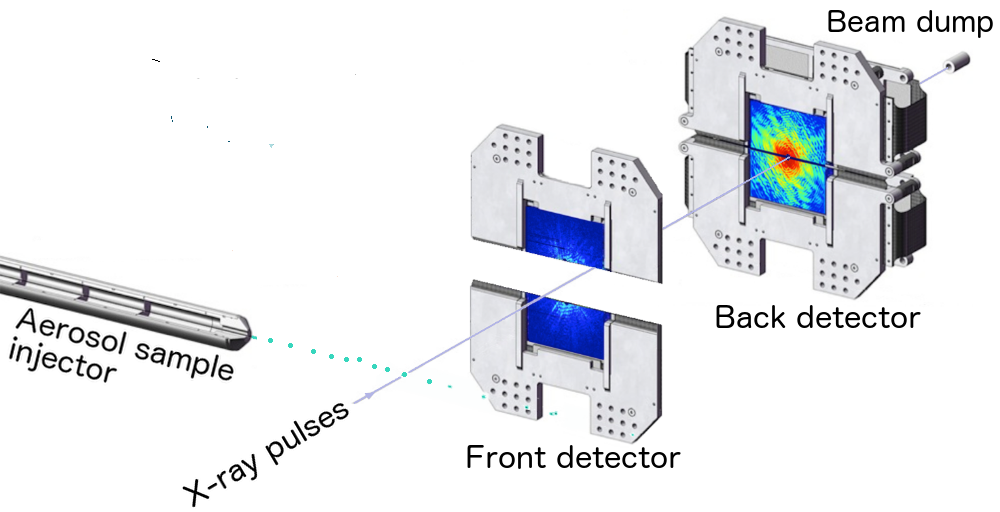
\includegraphics[width=90mm]{Geometry2.png}
\caption{The experimental geometry. Sample is introduced into the X-ray pulse train, using an aerosol sample injector. The diffracted signal is recorded on two pairs of detectors. The front detector pair is opened such that it does not shadow the back detector. The direct beam passes trough a central hole in the back detector.}\label{fig:experimental_geometry}
\end{figure}

$F(\vec{S})$ is independent from detector distance $d$, while a diffraction pattern is not. The relative scaling factor between the two is $\frac{1}{\lambda\,d}$. This means that the area covered by a pixel of size $p$ on the detector covers an area of size $q = \frac{p}{\lambda \, d}$ of the Ewald sphere (given the small angle approximation holds). 

Using the scaling relation between $F(\vec{S})$ sampled at the Ewald sphere, and the measured diffraction pattern at the detector, we can derive that pixel $P$ on the detector corresponds to pixel $\vec{Q} = \frac{\vec{P}}{\lambda\,d}$ on the Ewald sphere. 

Since $F(\vec{S})$ is measured at discrete locations, we have to use the discrete Fourier transform (DFT), and its inverse, to describe the relation between the measured diffraction pattern and the scattering potential. From now on we will use $F(\vec{Q})$ to describe $F(\vec{S})$ measured at discrete positions. 

The use of the DFT implies that the scattering potential is also discretized. The pixel size in real space (scattering potential space) $r$ is the inverse of the size of the detector in Fourier space ($D$). $D = n\,q$, where $n$ in the number of pixels on the detector, $q$ is the size of a pixel on the Ewald sphere. $q$ is the scaled version of a detector pixel: 
\begin{equation}\label{eq:q}
q = \frac{p}{\lambda d}
\end{equation}
This makes $r$:
\begin{equation}
r = \frac{\lambda\,d}{n\,p}
\end{equation}
Here $\lambda$ is the wavelength of the radiation, $d$ the detector distance, and $p$ is the size of a detector pixel.

%In a measurement the energy of a EM wave appears quantized, which means that one will always measure an integer number of the basic quantum of radiation: photons. The energy of a photon is related to its wavelength. The quantisation the measured intensity also has as an effect on the statistics, as they ar

\section{Missing Data}
The geometry of the detectors used in the experiments described in this thesis consist of two moveable halves (38.4 mm by 76.8 mm), with a dead area of at least 0.8 mm in between both halves (see figure \ref{fig:experimental_geometry}). In the center of the
detector a hole is created to let the high-intensity direct beam through (each detector half misses a semicircle). For both the dead area, and the central hole no intensity information is present, and the diffraction pattern is incomplete. 

In some experiments two pairs of detectors are used, in which one pair located closer to the sample (see figure \ref{fig:experimental_geometry}). The back detector is closed, and the front detector is opened such that it does not shadow the back detector. This opening results in a large area of missing data.
 
\section{Saturation}
Besides missing data due to the detector geometry, detector saturation might also lead to missing information. Each pixel on the detector can maximally hold a certain amount of electrical charge. If more charge is present in the pixel, the excess charge will overflow to neighbouring pixels, making it impossible to accurately use the original pixel as well as the affected pixels. If the amount of charge is very high, saturation might even damage the detector itself. Saturation usually occurs in the center of the detector, because these regions are typically the most intense regions of a diffraction pattern. 




